%\documentclass[numberedappendix,iop,12pt]{emulateapj}
%\documentclass{report}
\documentclass[12pt]{article}

\usepackage[legalpaper, margin=1.2in]{geometry}
\usepackage{graphicx} % Include figure files
\usepackage{dcolumn}% Align table columns on decimal point
\usepackage{bm}% bold math
\usepackage{epsf}
\usepackage{verbatim}
\usepackage{amsmath}
\usepackage{amssymb}
\usepackage[utf8]{inputenc}
\usepackage{appendix}
\usepackage{color}
\usepackage{soul}
\usepackage{verbatim} % needed for comments
%\usepackage[normalem]{ulem} % needed for strikeout font
\usepackage{mathtools}
%\usepackage{changes}
\usepackage{amsfonts}
\usepackage{tikz}
\usepackage{relsize}
\usepackage{natbib}
\usepackage{mhchem}
%\usepackage{multicol}
\usepackage{hyperref}% http://ctan.org/pkg/hyperref
\hypersetup{%
  colorlinks = true,
  linkcolor  = black,
  citecolor  = darkgreen
}


\usepackage{xcolor}
\usepackage[width=0.8\textwidth ,font={small, sf,it},labelfont={color=blue,bf},
labelsep=endash, format=plain,labelsep=period]{caption}

\definecolor{darkgreen}{rgb}{0.0,0.5,0.0}
%\usepackage[colorlinks,citecolor=darkgreen,dvipdfm]{hyperref} % Works with LaTeX, links fail in dvi.
% Add the next line only when strictly necessary, because it causes font bugs:
\usepackage[makeroom]{cancel}



% User defined commands:
\newcommand{\erf}{\mbox{erf}}
\newcommand{\fig}[1]{{#1}}
\def\myfig#1{#1}
%\def\myfig#1{}


\newcommand{\DrawFig}[1]{{#1}}
%\newcommand{\DrawFig}[1]{{}}


\def\mybib#1{./#1}


\newcommand{\cfixme}[1]{{\textcolor{red}{#1}}}
% Turn fixme, Fixme, cfixme  off before submission, e.g.
%\newcommand{\Fixme}[1]{{}}

\newcommand{\Uri}[1]{{\textcolor{orange}{#1}}}


\newcommand{\mathbfA}[1]{{\textbf{\mathbfmath{#1}}}}
\newcommand{\energain}{g}
\newcommand{\zeroeqconst}{\zeta}
\newcommand{\myPret}{P_{\tiny\text{ret}}}
\newcommand{\mysiso}{s_{\tiny\text{iso}}}
\newcommand{\myPesc}{P_{\tiny\text{esc}}}
\newcommand{\RPWN}{R_{\mbox{\tiny PWN}}}
\newcommand{\qdinf}{q_{\infty}}

\newcommand{\aaps}{AAPS}


\linespread{1.2}
\begin{document}

%\bibliographystyle{prsty} % Choose Phys. Rev. style for bibliography
%\submitted{M.Sc. thesis proposal ??}
\title{
\vspace{0cm}
\LARGE{{\bf Mean-field of $\ce{Ni(OH)_2}$ electrode in the Edison rechargeable battery} \\ \vspace{0.5cm}
{\Large Senior Year Physics Project}
\vspace{2cm}
}
}


\author{Submitted by: Nadav Porat \\ Advisor: Prof. Arik Yochelis }





%\affil{Physics Department, Ben-Gurion University of the Negev, POB 653, Be'er-Sheva 84105, Israel}



\date{\today}
\maketitle


%\onecolumngrid
%\onecolumn

\pagebreak
\tableofcontents
\pagebreak
\section{Introduction} 


\subsection{The problem with nickel-hydroxide electrodes} \label{sec:Nickel hydroxide}
Nickel-hydroxide is a compound of $\ce{Ni}$ and two hydroxide molecules $\ce{OH}$, making the substance $\ce{Ni(OH)_2}$. It is used as an electrode in rechargeable batteries (batteries that can be discharged and then charged again) like the Edison battery, which is much cleaner than the common Lithium battery because it doesn't involve toxic materials.
The basic function of the nickel-hydroxide electrode in a rechargeable battery is to store electrical charge and release it according to electrical and chemical changes. The nickel-hydroxide electrode accomplishes that by the following bidirectional chemical reaction \hyperlink{c:4}{[4]}:
\begin{equation} \label{eq:reaction}
    \ce{Ni(OH)_2 + OH^- <-> NiOOH + H_2O + e^- }
\end{equation} \label{eq:11}

This is a redox reaction. When the $\ce{NiOOH}$ compound gains an electron, it changes the composition of the electrode from nickel-hydroxide to nickel-oxide-hydroxide. We will refer to this change as a phase change in the electrode. A schematic illustration of the phases can be found in Figure \ref{fig:composition}.

\begin{figure}[h!] 
	\centering 
	\includegraphics[width=10cm,scale=1]{phase transition.jpg}
	\caption{Schematic illustration of the composition of $\ce{NiOOH}$ and $\ce{Ni(OH)_2}$, taken from \hyperref[c:4]{[4]}} \label{fig:composition}
\end{figure}

The problem with nickel hydroxide electrodes is that they are not effective enough for modern uses. In an ideal battery, all of the material undergoes a phase transition during charge/discharge. This process stops when one of the phases reaches the boundary. The hypothesised cause for the ineffectiveness is the development of "fingers" - spatially non-uniform phase transition. When one of those fingers reaches the boundary, the phase transition stops and some of the materiel remains non utilized. Previous efforts to model the electrode's characteristics does not take into account the spatial phase transformation and thus don't tackle the issue of instability \hyperref[c:5]{[5]}.
Therefore, \textbf{this project's goal is to provide a mathematical model that captures the spatial phase transformation of the nickel-hydroxide electrode}. Hopefully, this model will further the understanding of the electrode's dynamics and in turn the performance of the Edison battery.


\subsection{Typical battery structure} \label{sec:batt}
Batteries store electrical energy using chemical reactions (redox reactions). In a typical battery, the energy conversion takes place inside units called electrochemical "cells" which are connected in some pattern to a circuit. A cell typically consists of three components: positive electrode (cathode), negative electrode (anode), and an electrolyte. A porous barrier is placed between the cathode and anode which allows movement of ions but not of electrons. An illustration of a cell can be found in Figure \ref{fig:battery}.

\begin{figure}[h!] 
	\centering 
	\includegraphics[width=6cm,scale=0.6]{battery.jpg}
	\caption{Schematic illustration of a typical electrochemical cell, from \hyperref[c:6]{[6]}} \label{fig:battery}
\end{figure}

The electrodes are a solid metallic compound that can hold ions, the electrolyte is usually a solution of water and other solvents. The anode holds the electrons in an energy level that is "high enough to escape the material", but when the battery is not connected to a closed circuit, the electrons have "no where to go". When a closed circuit is formed with the battery, the electrons "escape" to the circuit and flow to the cathode, thus creating an electric current. At the same time, the ions dissolve in the electrolyte and are pulled through the porous barrier to the cathode. 

From the description above, we can deduce the general forces that occur in the electrode while charging/discharging and apply them to nickel-hydroxide. First, we have \textit{charge transport} of the ions in the solution and the electrons in the material. Second, there are \textit{electric forces} that influence the electrons in the electrode. Lastly, the electrode's materiel goes through a \textit{phase transition} when it loses ions or electrons (reaction (\ref{eq:reaction})). In the following text, we will provide equations for these dynamics and build upon them a mathematical model for the nickel-hydroxide electrode.


\subsection{Charge transport - Poisson-Nernst-Planck} \label{sec:pnp}
 In this subsection, we will derive the Poisson-Nernst-Planck model to tackle the \textit{charge transport}, and \textit{electric forces} that are mentioned at the end of the \hyperref[sec:batt]{Batteries} section.
 
 One of the core physical components that make up batteries is charge transport in a solution. The movement is induced by two physical processes: thermodynamic diffusion and electrical migration (while neglecting convection $v$). The diffusion is caused due to a concentration difference, and the migration due to electric potential difference.

Following \hyperref[c:2]{[2]}, consider a box with dimensions $(L_x, L_y, L_z)$ filled with water and ion species $(j=1,2...N)$. Each ion species $j$ has an electrochemical potential that is a function of time and space, denoted by $\mu_j (t, \bf{r})$. According to thermodynamics, a  difference in the electrochemical potential between two points, $\mu_j (t, {\bf r_1}) < \mu_j (t, {\bf r_2})$, will create a flux of species $j$ to lessen said difference. The flux is proportional to the gradient of $\mu_j$ and concentration of species $j$, $c_j$ at the point:
\begin{equation} \label{eq:ion-flux}
    {\bf J}_j (t, {\bf r}) = -\frac{D}{k_B T} c_j(t, {\bf r}) \nabla \mu_j(t, {\bf r})  
\end{equation}
with $D, k_B, T$ the diffusion constant, Boltzmann constant, and temperature (we assume constant temperature and identical diffusion constants). 
Basic thermodynamics tells us that the electrochemical potential can be described by:
\begin{equation}
    \mu_j(t, {\bf r}) = k_B T \ln c_j (t, {\bf r}) + z_j \phi (t, {\bf r})    
\end{equation}
where $z_j, \phi$ are the valance of species $j$, and electric potential. Substituting into the flux (\ref{eq:ion-flux}):
\begin{equation}
    {\bf J}_j (t, {\bf r}) = -D \nabla c_j -\frac{Dz_j}{k_BT} c_j\nabla \phi    
\end{equation}
where we omitted the function arguments for simplicity. 
The flux is substituted into the transport (continuity) equation:
\begin{equation} \label{eq:continuity}
    \frac{\partial c_j (t, {\bf r})}{\partial t} = -\nabla \cdot \bf{J_j}(t, {\bf r})    
\end{equation}
and results in the Nernst-Planck equation (in the absence of advection):
\begin{equation} \label{eq:nernst-planck}
\frac{\partial c_j (t, {\bf r})}{\partial t} = \nabla \cdot \left[ D \nabla c_j(t, {\bf r}) +\frac{Dz_j}{k_BT} c_j(t, {\bf r}) \nabla \phi (t, {\bf r}) \right]
\end{equation}

As we can see, the Nernst-Planck equation is a differential equation that describes the motion of ions 
subjected to diffusion and electric potential. Notice that the equation contains the regular diffusion equation (the first term on the RHS).

The electric potential is governed by the Poisson equation:
\begin{equation}
    -\nabla \cdot (\epsilon \nabla \phi(t, {\bf r})) = 4 \pi \rho (t, {\bf r})   
\end{equation}
 with $\rho$ being the charge density. In our case, $\rho$ is the charge-carrier concentrations $c_j$:
\begin{equation} \label{eq:poisson}
    -\nabla \cdot (\epsilon \nabla \phi(t, {\bf r})) = 4\pi \sum _{j=1} ^N z_j c_j (t, {\bf r})  
\end{equation}
\newline 
The Poisson equation (\ref{eq:poisson}), together with the $N$ Nernst-Planck equations (one for each species) (\ref{eq:nernst-planck}), constitute the Poisson-Nernst-Planck model. It's a system of PDE's that describes the movement of charge-carriers in a solution subjected to an electric gradient. An optional finite-difference numerical solution for the 1D PNP model is presented in \hyperref[sec:appendix-a]{Appendix A}.

We will use this model in the \hyperref[sec:model-equations]{Model equations section} to describe the dynamics of the electrons in the nickel-hydroxide battary. 

\subsection{Phase separation - Cahn-Hilliard approach} \label{sec:Cahn-Hilliard}
 In this subsection, we will derive Cahn-Hilliard like equations to tackle the \textit{phase separation} that is mentioned at the end of the \hyperref[sec:batt]{Batteries} section.

We want to describe a system with two species (or phases), $A$ and $B$, where the phases are mixed at first and over time they separate, like oil and water, or the illustration in Figure \ref{fig:cahn-hilliard}. The interaction energies determines which state is preferred, one where particle $A$ is interacting with another $A$ particle, or with a $B$ particle. Phase separation requires that the $A-B$ interaction would be less preferable, i.e. higher energetic value. We will incorporate that into the free energy, so that we could then use it to derive $\mu_i$ and an equation for $\bf J_i$, with $i=A,B$. 
\newline \newline \newline \newline

\begin{figure}[h!] 
	\centering 
	\includegraphics[width=6cm,scale=0.8]{cahn hilliard example.png}
	\caption{Schematic illustration of the progression of Chan-Hilliard equations in 2D. At first the two phases (blue and yellow) are well mixed, and with time they tend to separate. From \hyperref[c:7]{[7]}} \label{fig:cahn-hilliard}
\end{figure}

Following \hyperref[c:3]{[3]}, assume we have a system with two species $A, B$ and pairwise interaction energies: $E_{AA}, E_{BB}, E_{AB}$. The local concentrations of the species in the system are denoted $c_A(t, {\bf r}), c_B(t, {\bf r})$. Since they satisfy mass conservation $c_A + c_B = 1$, we can define a symmetric variable $u$ as $u = c_A - c_B$. The range of $u$ is $[-1,1]$, such that $u=1$ for pure $A$ phase and $u=-1$ for pure $B$ phase. The interactions $AA$ and $BB$ are preferable to $AB$, so we require $E_{AB} > E_{AA}, E_{BB}$.

We achieve this requirement by adding an "energy penalty" to the free energy. The penalty would be given according to concentration differences between the two species, meaning $\nabla u(t, {\bf r})$. But the direction of the change doesn't matter to our purposes, only its magnitude, so the energetic penalty would be proportional to $|\nabla u|^2$. 

This penalty is not enough, however. It vanishes for a spatially constant mixed state (say $u({\bf r}) \approx 0$) but we want this state to be unfavorable. Therefore we add another term - $W(u)$. The function $W$ is system dependent, it should produce high values for our undesired states ($|u| \approx 0$), and low values for our desired states ($|u| \approx 1$).

Combining both terms, the free energy functional $\mathcal{F}[u(t, {\bf r})]$ takes the form:
\begin{equation}
    \mathcal{F}[u(t, {\bf r})] = \int \beta W(u) + E_0 |\nabla u|^2 \, d{\bf r}
\end{equation}
where we added $\beta, E_0$ as proportionality constants.

The chemical potential $\mu$ is the variation of the free-energy, $\frac{\delta \mathcal{F}}{\delta u} = \mu$. We'll use the Euler-Lagrange formulation,
\begin{equation}
   \mu = \frac{\delta \mathcal{F}}{\delta u} = \frac{\partial f}{\partial u} - \nabla \cdot \left(\frac{\partial f}{\partial (\nabla u)}\right)
\end{equation}
where $f$ is the integrand of $\mathcal{F}$.
Finally, we'll substitute $\mu$ into the flux definition $J$ (\ref{eq:ion-flux}) and continuity equation (\ref{eq:continuity}):
\begin{equation} \label{eq:cahn-hilliard}
    \frac{\partial u}{\partial t} = \frac{D}{k_B T} \nabla \cdot \left[  \beta W''(u) \nabla u - 2E_0 \nabla ^3 u \right]
\end{equation}

Equation (\ref{eq:cahn-hilliard}) together with an appropriate $W$ function that will be defined in the  \hyperref[sec:model-equations]{Model equations section}, describes our desired phase separation dynamics.


\pagebreak
\section{Model equations} \label{sec:model-equations}

\subsection{Construction of free energy}
Our goal is to model the nickel-hydroxide to nickel-oxide-hydorxide electrochemical reaction (\ref{eq:reaction}) which is taking place in the electrode. We begin by formulating the free energy of the nickel-hydroxide electrode. The substance $\ce{NiOOH}$ is denoted as phase $A$, and substance $\ce{Ni(OH)_2}$ as $B$. Following the the \hyperref[sec:Cahn-Hilliard]{Chan-Hilliard approach}, we define $u(t, {\bf r})=c_B(t, {\bf r})-c_A(t, {\bf r})$ as the order parameter, so its range is $[-1,1]$, where $u=1$ means a pure $\ce{Ni(OH)_2}$ phase and $u=-1$ is a pure $\ce{NiOOH}$ phase.
We divide the free-energy into three contributions:

\begin{equation}
    \large \varepsilon = \varepsilon_{mixing} + \varepsilon_{entropy} + \varepsilon_{electric}
\end{equation}

The mixing energy:
\begin{equation}
     \varepsilon_{mixing} = c\int \beta W(u) + \frac{1}{2} E_0 \kappa^2 |\nabla u|^2 \, d{\bf r}
\end{equation}
where $c$ is a reference density, $\beta$ is a phase interaction parameter with energy units, $E_0$ has energy units and $\kappa$ has length units. 

$W(u)$ is the mixing penalty described in the \hyperref[sec:Cahn-Hilliard]{Cahn-Hilliard section}, it needs to account for the inclination of the material to be in one of two pure states. Therefore, $W$ is a double-well function:
\begin{equation} \label{eq:wu}
    W(u) = au^4 - bu^2
\end{equation}
where $a, b$ are parameters that are set and optimized during numerical analysis. The function's behaviour is described in Figure \ref{fig:wu}. 

\begin{figure}[h!] 
	\centering 
	\includegraphics[width=7cm,scale=1]{wu.jpg}
	\caption{Chan-Hilliard penalty function $W(u)$ (\ref{eq:wu}) with $a=2.5, b=-4.4$} \label{fig:wu}
\end{figure}

The electrons are the mobile-charges of the system, their charge density is denoted by $n(t, {\bf r})$. They contribute to the electrostatic energy along with the energy density $- \frac{1}{2}\epsilon|\nabla \phi|^2$:

\begin{equation}
    \varepsilon_{electric} = \int -qn\phi - \frac{1}{2}\epsilon|\nabla \phi|^2 \, d{\bf r}
\end{equation}
where $q$ is the elementary charge. 


Finally, the thermodynamic energy arises from the entropy of the material and charges:

\begin{equation}
    \varepsilon_{entropy} = k_BT \int c\frac{1-u}{2}\ln{\frac{1-u}{2}} + c\frac{1+u}{2}\ln{\frac{1+u}{2}} + n\ln{\frac{n}{c}} \, d{\bf r}
\end{equation}

\subsection{Integration of PNP equations}
As mentioned in the \hyperref[sec:Cahn-Hilliard] {Cahn-Hilliard section}, we can derive the fluxes $\mathbf{J}^u, \mathbf{J}^n$ using variation on the free-energy $\varepsilon$. The Poisson equation is also accounted for with a variation. Afterwards, we'll use the \hyperref[sec:pnp]{Poisson-Nernst-Planck} model to describe the dynamics of the charge-transport in the system. 

Using the continuity equation (\ref{eq:continuity}):
\begin{equation}
    \begin{aligned}
        \frac{\partial u}{\partial t} &= \nabla \cdot \mathbf{J}^u = \nabla \cdot \left( \frac{D_u}{ck_BT}(1-u^2)\nabla \frac{\delta \varepsilon}{\delta u} \right)\\
        \frac{\partial n}{\partial t} &= \nabla \cdot \mathbf{J}^n = \nabla \cdot \frac{D_n}{k_BT}n \nabla \frac{\delta \varepsilon}{\delta n}
    \end{aligned}
\end{equation}
Note that, with accordance to \hyperref[c:1]{[1]}, we added an $(1-u^2)$ component that keeps $u$ in the appropriate range.

Using calculus of variations' notation:
\begin{equation}
   \frac{\delta J}{\delta y(x)} = \frac{\partial f}{\partial y} - \frac{d}{dx} \left(\frac{\partial f}{\partial y'}\right), \, J[y] = \int f(x, y, y') \, dx
\end{equation}
we derive the following fluxes:
\begin{equation} \label{eq:base-model1}
    \begin{aligned}
        n\nabla \frac{\delta \varepsilon}{\delta n} &= - qn\nabla \phi + k_B T\nabla n \\
        \nabla \frac{\delta \varepsilon}{\delta u} &= c\beta W''(u) \nabla u + cE_0 \kappa^2 \nabla^3 u + k_B T c \frac{\nabla u}{1-u^2}
    \end{aligned}
\end{equation}
and Poisson's equation:
\begin{equation} \label{eq:base-model2}
    0 = \frac{\delta \varepsilon}{\delta \phi} = -nq + \nabla \cdot (\epsilon \nabla \phi)
\end{equation}

\subsection{Dimensionless units}

In order to solve the model numerically, we want to bring the equations into their pure mathematical form. Therefore, we will do the following rescaling:
\begin{equation}
    \begin{aligned}
        \mathbf{\tilde{x}} &= \frac{\mathbf{x}}{l},  \tilde{n} = \frac{n}{c}, \tilde{\phi} = \frac{q}{k_BT}\phi \\
        \tilde{\beta} &= \frac{\beta}{k_BT}, \tilde{\epsilon} = \frac{k_BTl}{q^2}\epsilon, \lambda = \frac{E_0}{k_BT} \frac{\kappa^2}{l^2}
    \end{aligned}
\end{equation}
and remove the tildes. Eventually we get from (\ref{eq:base-model1}), (\ref{eq:base-model2}):

\begin{subequations}\label{eq:dimensionless-model}
    \begin{align}
        \frac{\partial n}{\partial t} &= \nabla \cdot D_n( \nabla n - n\nabla \phi) \\
        \frac{\partial u}{\partial t} &= \nabla \cdot D_u (1-u^2) \cdot \left[\frac{1}{1-u^2}\nabla u + \beta W''(u)\nabla u +\lambda \nabla ^3 u\right] \\
    0 &= -n + \nabla \cdot (\epsilon \nabla \phi)
    \end{align}
\end{subequations}

\subsection{Electron interaction with Ni phases} \label{sec:electron-material}
Up until now we treated the material $u$ and the electrons $n$ as if they were not interacting - each was governed by a separate set of laws. However, the phase transfer introduced in the \hyperref[sec:Nickel hydroxide]{Nickel hydroxide section} changes the electron's concentration $n$ and the phase "concentration" $u$.

We will account for this interaction using the fact that reaction (\ref{eq:reaction}) is spontaneous. Therefore, if the $\ce{NiOOH}$ phase ($u=-1$) is present in an environment with high electron concentration ($n$), it will spontaneously transform into the $\ce{Ni(OH)_2}$ phase ($u=1$) while reducing the electron concentration. When the electron concentration is low and phase $\ce{Ni(OH)_2}$ is present, the phase would change in the opposite direction and the electron concentration would increase. This process is introduced to the model with the following term:

\begin{equation}
    I = \alpha \frac{1}{2} \big( (1-u)n - (1+u)(1-n) \big)
\end{equation}
where $\alpha$ is the rate of the transition (in Hz). $I$ is added to the $\partial_t u$ equation with a positive sign and to the $\partial_t n$ equation with a negative sign.

Finally, together with (\ref{eq:dimensionless-model}), we get the full, dimensionless model:
\begin{subequations} \label{eq:full-model}
    \begin{align} 
        \begin{split}
        \frac{\partial u}{\partial t} ={}& \nabla  \cdot D_u (1-u^2) \cdot \left[ \frac{1}{1-u^2}\nabla u + \underbrace{\beta W''(u)\nabla u + \lambda \nabla ^3 u}_{\text{phase separation}} \right] \\
        & + \underbrace{\frac{\alpha}{2} \big( (1-u)n - (1+u)(1-n) \big)}_{\text{phase transition}}
        \end{split}\\
        \frac{\partial n}{\partial t} ={}& \underbrace{\nabla \cdot D_n(\nabla n - n\nabla \phi)}_{\text{migration-diffusion}} - \frac{\alpha}{2} \big( (1-u)n - (1+u)(1-n) \big)\\
    0 ={}& -n + \nabla \cdot (\epsilon \nabla \phi)
    \end{align}
\end{subequations}

The model's fluxes are denoted as:  
\begin{align} \label{eq:full-model-vector-notation}
    \begin{bmatrix}
        {\bf J}_{\phi} \\
        {\bf J}_n \\
        {\bf J}_u 
    \end{bmatrix}
    &= \begin{bmatrix}
        \nabla \epsilon \phi \\
        \nabla n - n \nabla \phi \\
        (1-u^2) \left[ \frac{1}{1-u^2} \nabla u + \beta W''(u) \nabla u + \lambda \nabla \psi \right] 
   \end{bmatrix}
\end{align}

And the boundary-conditions for the input electron flux case:
\begin{equation}\label{eq:full-model-bo}
    \begin{aligned}
        \phi(t, {\bf r}_L) &= \phi(t, {\bf r}_R) = 0 \\
        {\bf J}_u(t, {\bf r}_L) &= {\bf J}_u(t, {\bf r}_R) = 0 \\
        {\bf J}_n(t, {\bf r}_L) &= 0, \,  {\bf J}_n(t, {\bf r}_R) = -a
    \end{aligned}
\end{equation}
where ${\bf r}_L, {\bf r}_R$ denote the left and right edges of the electrode, and $a$ is some nonzero charging rate.

Equations (\ref{eq:full-model}) with the boundary conditions (\ref{eq:full-model-bo}) constitute this project's model for the nickel-hydroxide electrode.

\pagebreak
\section{Numerical analysis} \label{seq3}
\subsection{Numerical model} \label{sec:numerical-model}
The numerical solution was done in 1D using MATLAB's pedpe package, the full code is available in the project's \href{https://github.com/nadav7679/phase_field_Ni_batteries/tree/main/matlab/nickel}{Git repository}. MATLAB's pdepe does not allow  explicit 3rd or higher order derivatives, so to answer the package's constraints and implement the \hyperref[sec:Cahn-Hilliard] {Cahn-Hilliard} fourth-order derivative, we introduced a variable $\psi$ which is the second derivative of $u$. Afterwards, the numerical model (\ref{eq:full-model}) takes the following form in 1D:   

\begin{subequations} \label{eq:numerical-model}
    \begin{align}
        0 ={}& -n + \partial_x (\epsilon \partial_x \phi)\\
        \frac{\partial n}{\partial t} ={}& D_n \partial_x \cdot (\partial_x n - n \partial_x \phi) - \frac{\alpha}{2} \big( (1-u)n - (1+u)(1-n) \big)\\
        \begin{split}
        \frac{\partial u}{\partial t} ={}& D_u \partial_x \cdot (1-u^2) \left[ \frac{1}{1-u^2} \partial_x u + \beta W''(u) \partial_x u + \lambda \partial_x \psi \right] \\
        & + \frac{\alpha}{2} \big( (1-u)n - (1+u)(1-n) \big)
        \end{split}\\
        \psi ={}& \partial_x ^2 u
    \end{align}
\end{subequations}

The vector notation (\ref{eq:full-model-vector-notation}) becomes:  
\begin{align}
    \begin{bmatrix}
        J_{\phi} \\
        J_n \\
        J_u \\
        J_{\psi}
    \end{bmatrix}
    &= \begin{bmatrix}
        \partial_x \epsilon \phi \\
        \partial_x n - n \partial_x \phi \\
        (1-u^2) \left[ \frac{1}{1-u^2} \partial_x u + \beta W''(u) \partial_x u + \lambda \partial_x \psi \right] \\
        \partial_x \psi
   \end{bmatrix}
\end{align}
Additionally, we will denote the x-domain as $[x_L, x_R]$, which is taken to be $[-10, 10]$ in the simulations.

Finally, the parameter values for the simulations are given in \hyperref[table:1]{table 1}.
\begin{table}[h!]
\centering
\begin{tabular}{|c|c|} 

 \hline
 $D_u$ & 1  \\ 
    \hline
  $D_n$ & 1  \\ 
    \hline
 $\alpha$ & 1  \\ 
    \hline
  $\epsilon$ & 50  \\ 
    \hline
  $\beta$ & 1  \\ 
    \hline
  $\lambda$ & 3  \\ 
 \hline
\end{tabular} \label{table:1}
\caption{Parameter values}
\end{table}


\pagebreak
\subsection{Steady state solution}
The numerical model in (\ref{eq:numerical-model}) was implemented in MATLAB with Neumann boundary conditions for $u$ and $n$, and Dirichlet for $\psi$ and $\phi$:

\begin{equation}\label{eq:steady-state-bo}
    \begin{aligned}
        \phi(t, x_L) &= \phi(t, x_R) = 0 \\
        J_n(t, x_L) &= J_n(t, x_R) = 0 \\ 
        J_u(t, x_L) &= J_u(t, x_R) = 0 \\
        \psi(t, x_L) &= \psi(t, x_R) = 0 \\
    \end{aligned}
\end{equation}
These boundary conditions simulate a closed system - no electrons enter or exit the electrode, and both ends are fixed at the same voltage. The initial conditions of the simulation are such that the electrode is spatially divided into two almost-pure phases, right at the middle. The electron's concentration is divided in the same way. Initial and final graphs of the system are shown in Figure \ref{fig:steady-state}.

\begin{figure}[h!] 
	\centering 
	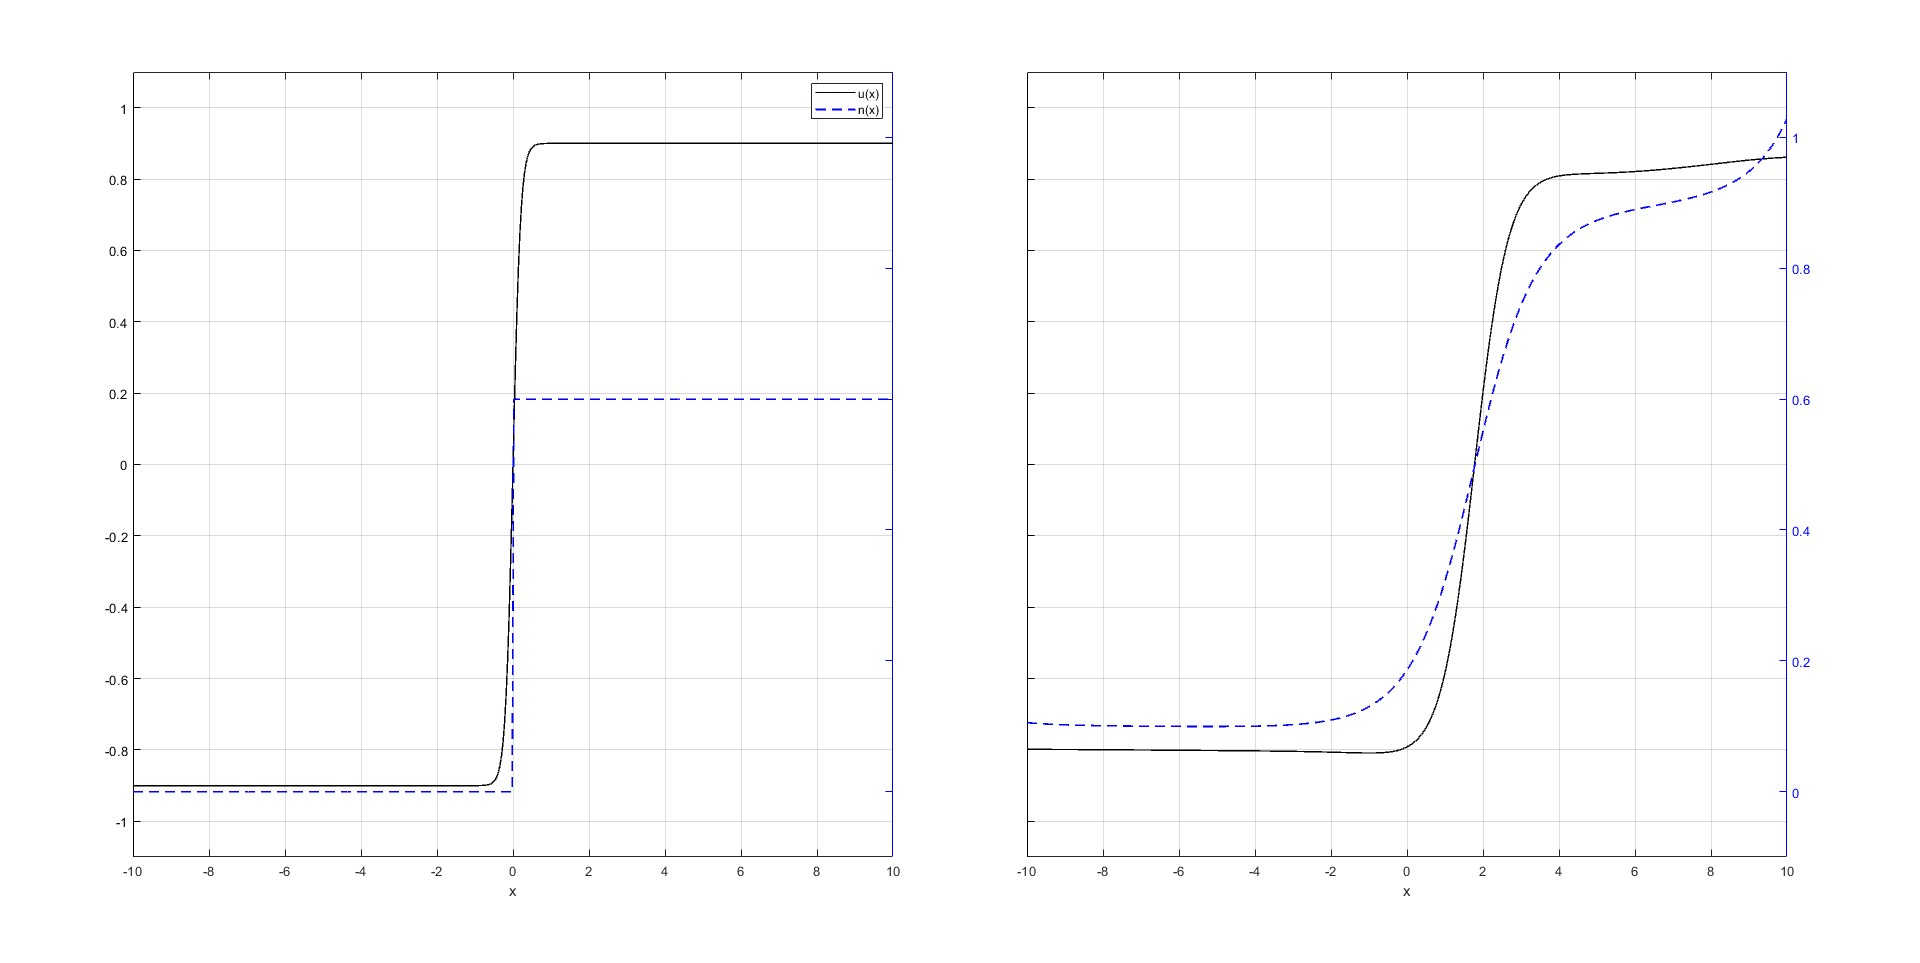
\includegraphics[width=15cm,scale=1]{steady state.jpg}
	\caption{Steady State solution of the numerical model with BC described in (\ref{eq:steady-state-bo}). A - initial state of the system, B - stable final state. We can see that $n(x)$ roughly follows $u(x)$.  } \label{fig:steady-state}
\end{figure}

Note that the acquired steady-state is not physical, as it depicts a state where half of the electrode is charged and the other half does not. In reality, both phases are neutral, so the high electron concentration that is present in Figure \ref{fig:steady-state} is either balanced out with another charge-carrier, decoupled from the material, or distributed in a different way.
With that being said, it is still worthwhile to examine the results and see that the numerical model produced a stable system which is halved into two phases by an interface. Additionally, as expected, the electron concentration roughly follows the "concentration" of the $\ce{Ni(OH)_2}$ phase. 
Notice that the electron concentration exceeds 1 at the right end of the final system state. This problem is a manifest of the potential BC in the numerical simulation, the electrons migrate towards the right end because its potential is fixed at zero, which results in a higher than one concentration.

Surprisingly, supplying an uneven $W(u)$ does not move the interface, even when the difference between the minimum points is large. However, the distance between the minimum $u$ values and $|u|=1$ does affect the plateau values of $u$, e.g. a minimum of $W$ with $0<u<0.5$ would result in a plateau ("pure" state value) with a $0<u<0.5$ value. $W$ also affects the shape of the final interface, sharper potential wells result in a sharper transition between the phases.

The initial concentration of $n$ does affect the location of the interface. A low concentration of electrons would allow the $\ce{NiOOH}$ phase to "take over" more space than $\ce{Ni(OH)_2}$, as we can see in Figure \ref{fig:low-n-ss}.

\begin{figure}[h!] 
	\centering 
	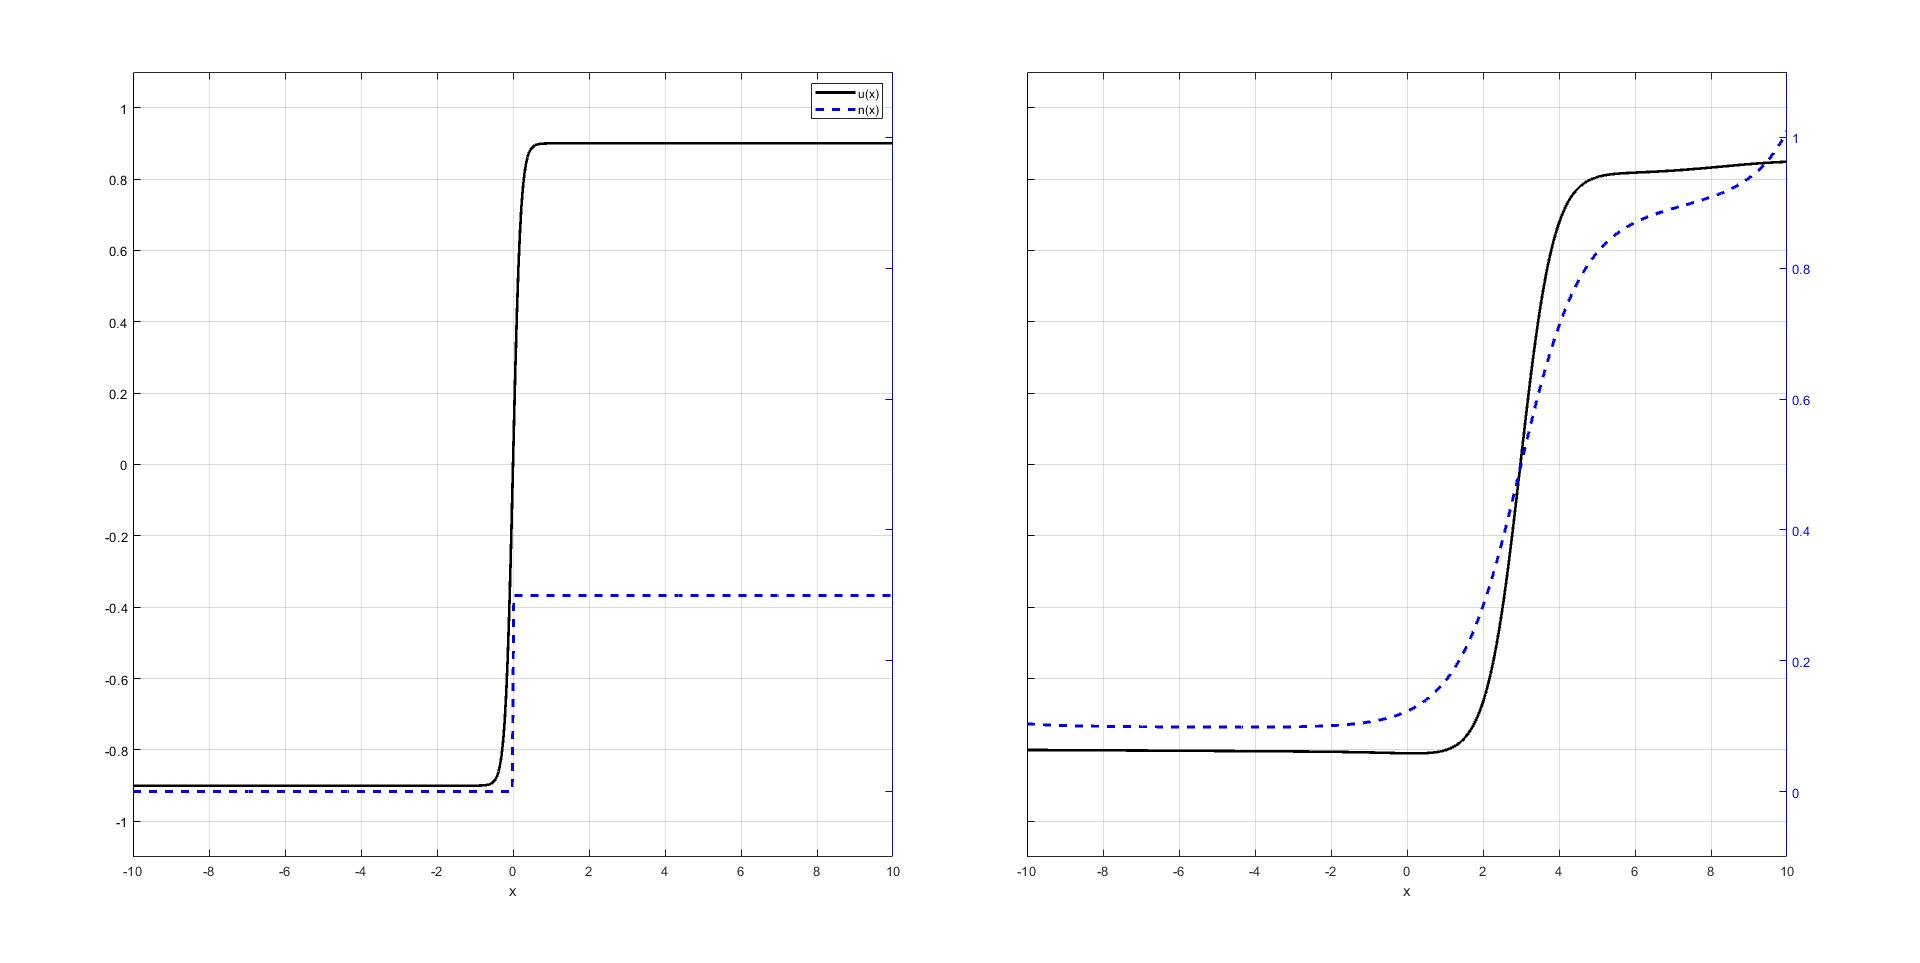
\includegraphics[width=15cm,scale=1]{low n steady state.jpg}
	\caption{Steady state solution with a low initial electron concentration $n$. A - initial state, interface at $x=0$. B - final state, interface moved to around $x=2.5$.} \label{fig:low-n-ss}
\end{figure}

\pagebreak
\subsection{Charging and discharging solutions}
Charging was simulated with an input electron flux to the electrode. Note that in this section we define $\ce{Ni(OH)_2}$ as the charged phase (because it's filled with negative charge), contrary to the usual definition.  We used the numerical model introduced in (\ref{eq:numerical-model}) and the boundary conditions described in (\ref{eq:steady-state-bo}), except for the $J_n$ BC which was set as follows:
\begin{equation}
    J_n(t, x_L) = 0, \, J_n(t, x_R) = -0.001
\end{equation}
The direction of the flux is set by its sign, and the magnitude was determined to be low enough so that the electrons could diffuse and won't build up near the edge.

Discharging was simulated with the same numerical model equations and the boundaries in (\ref{eq:steady-state-bo}), only this time the $J_n$ BC was was set to:
\begin{equation}
    J_n(t, x_L) = 0.001, \, J_n(t, x_R) = 0
\end{equation}

Results of the charging and discharging simulations are presented in Figure \ref{fig:input-flux} and Figure \ref{fig:output-flux} respectfully. We can see that in both cases one of the two pure phases took over the entire domain, which fits our physical problem. The interface translates with a constant speed, except for the beginning (ending) of the transition, where an acceleration (deacceleration) occurs. 


\begin{figure}[!h] 
	\centering 
	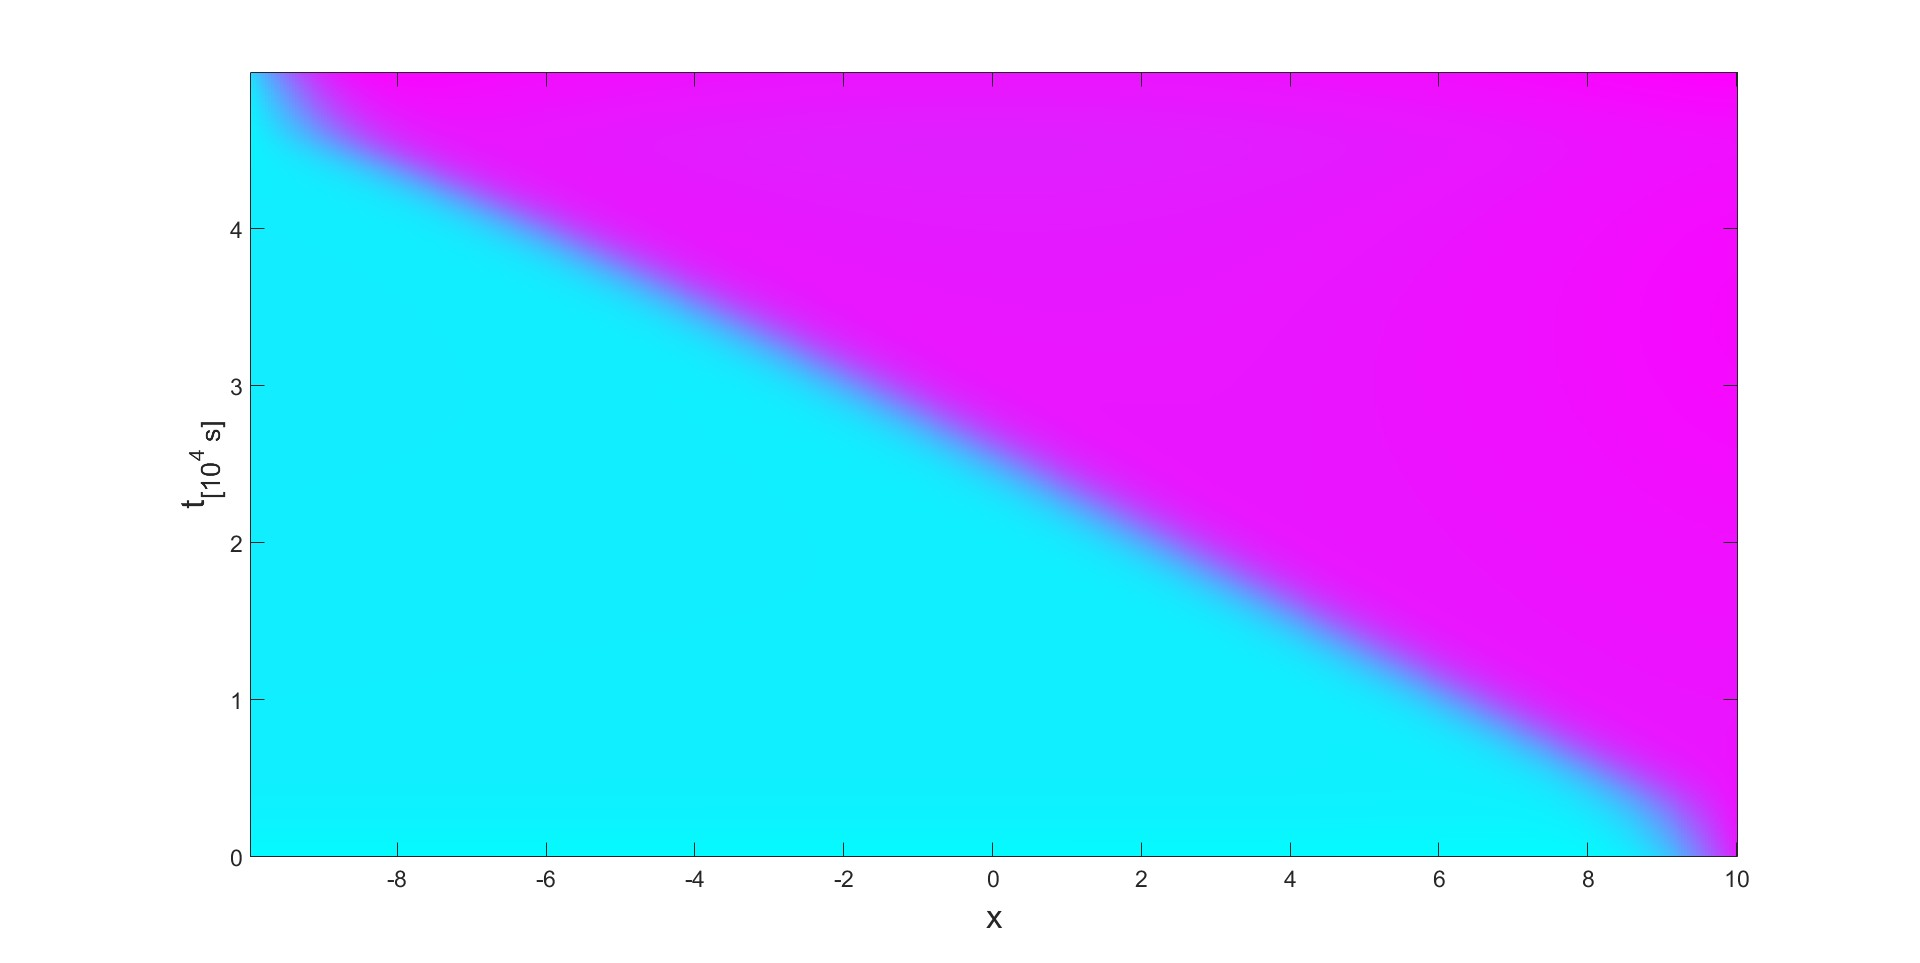
\includegraphics[width=15cm,scale=1]{input charge space time plot.jpg}
	\caption{Space-time plot with an input electron flux from the right. Purple - $\ce{Ni(OH)_2}$, Blue - $\ce{NiOOH}$. Over time, the $\ce{Ni(OH)_2}$ phase takes over the material and the interface moves to the left edge.} \label{fig:input-flux}
\end{figure}

\begin{figure}[!h] 
	\centering 
	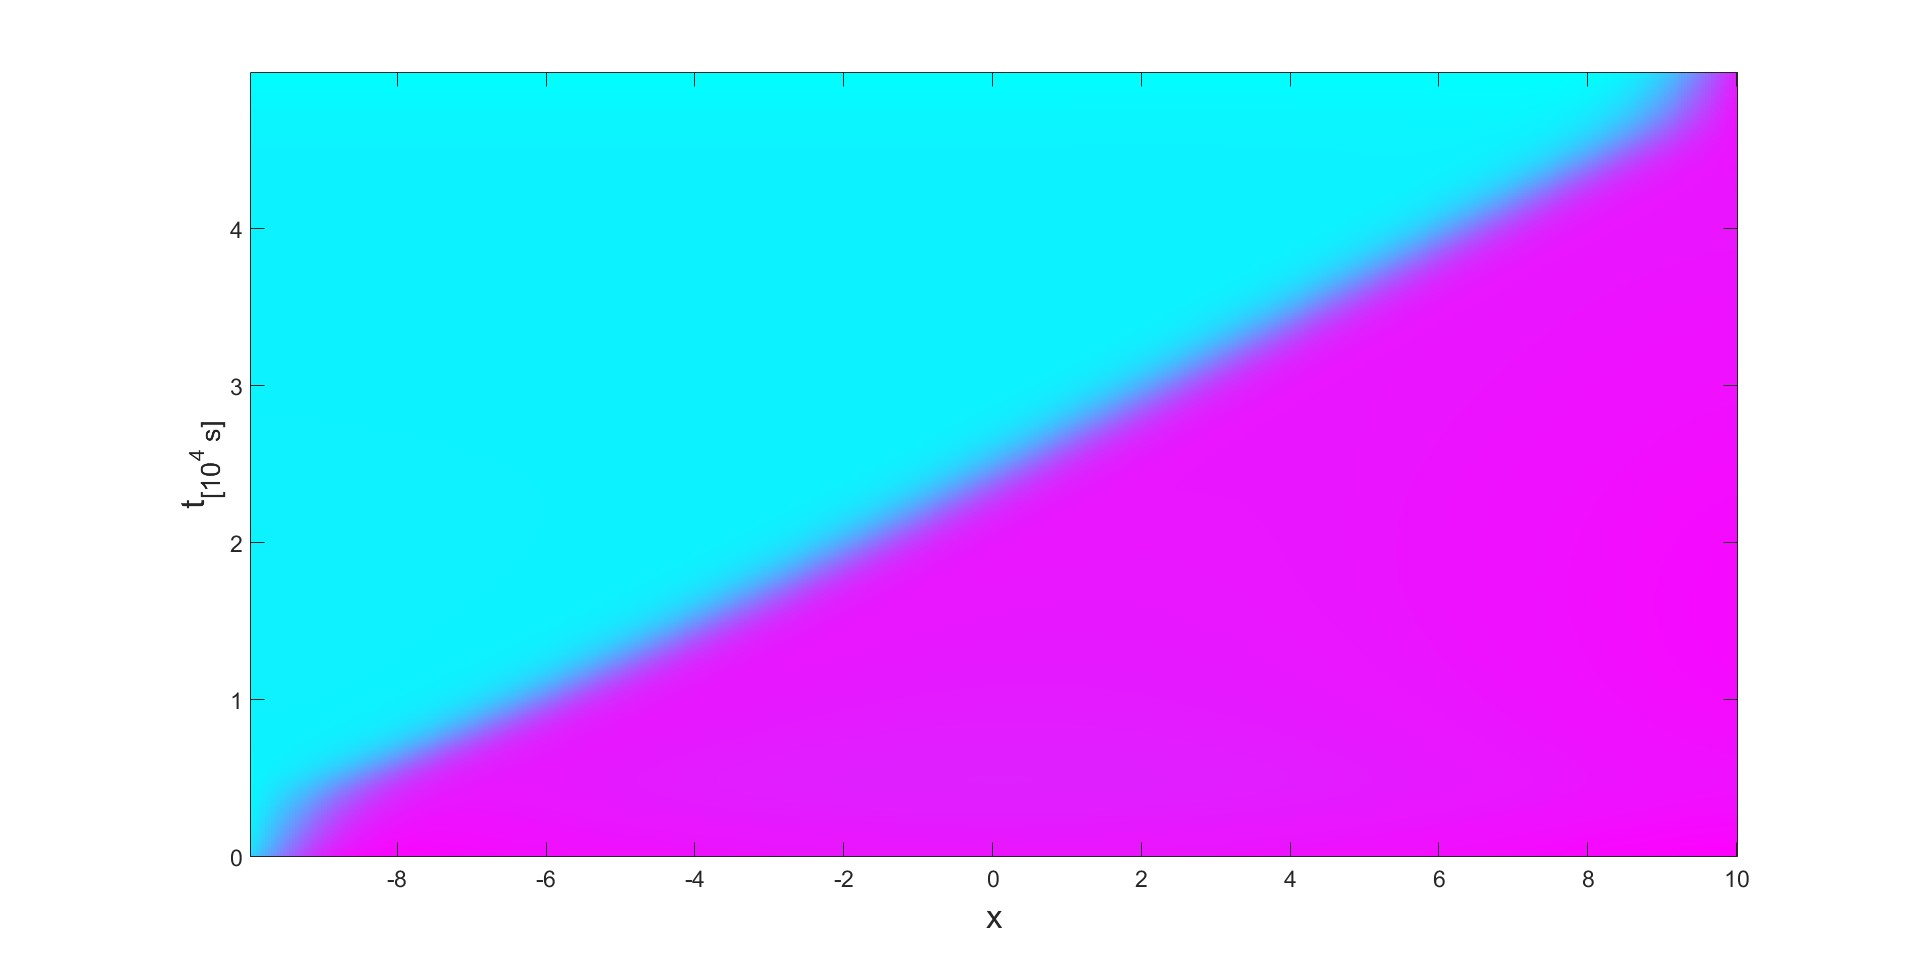
\includegraphics[width=15cm,scale=1]{output charge space time plot.jpg}
	\caption{Space-time plot with an output electron flux from the left. Purple - $\ce{Ni(OH)_2}$, Blue - $\ce{NiOOH}$. Over time, the $\ce{NiOOH}$ phase takes over the material and the interface moves to the right edge.} \label{fig:output-flux}
\end{figure}

Looking at the final electron distribution and $u$ profile at the end of the charged case can be worthwhile, it is presented in Figure \ref{fig:output-flux-solution}. As opposed to the discharge $u$ and $n$ profiles (not presented), the material is not at a fully pure phase in the middle of the domain ($u \approx 0.9$). This phenomenon can be related to the repelling forces between the electrons. These forces won't let them reach a high concentration ($n=1$) at the middle of the domain, so the charged phase is not as pure as it could be. In contrast, the discharging state does achieve its pure form.

Also in the charging case, we yet again get electron concentration values that are larger than 1. Once again it is a numerical problem - in the simulation the electron flux continued to flow in even though all of the material transformed, resulting in a diverging electron concentration.

Moreover, the simulation does not manage to create an interface from a pure domain-wide phase. If we apply the charging or discharging BC on initial conditions that consists of a domain-wide pure phase, we receive different phase separation behaviours that are different from an interface, e.g. parabolic behaviour, or a double interface.

\begin{figure}[h!] 
	\centering 
	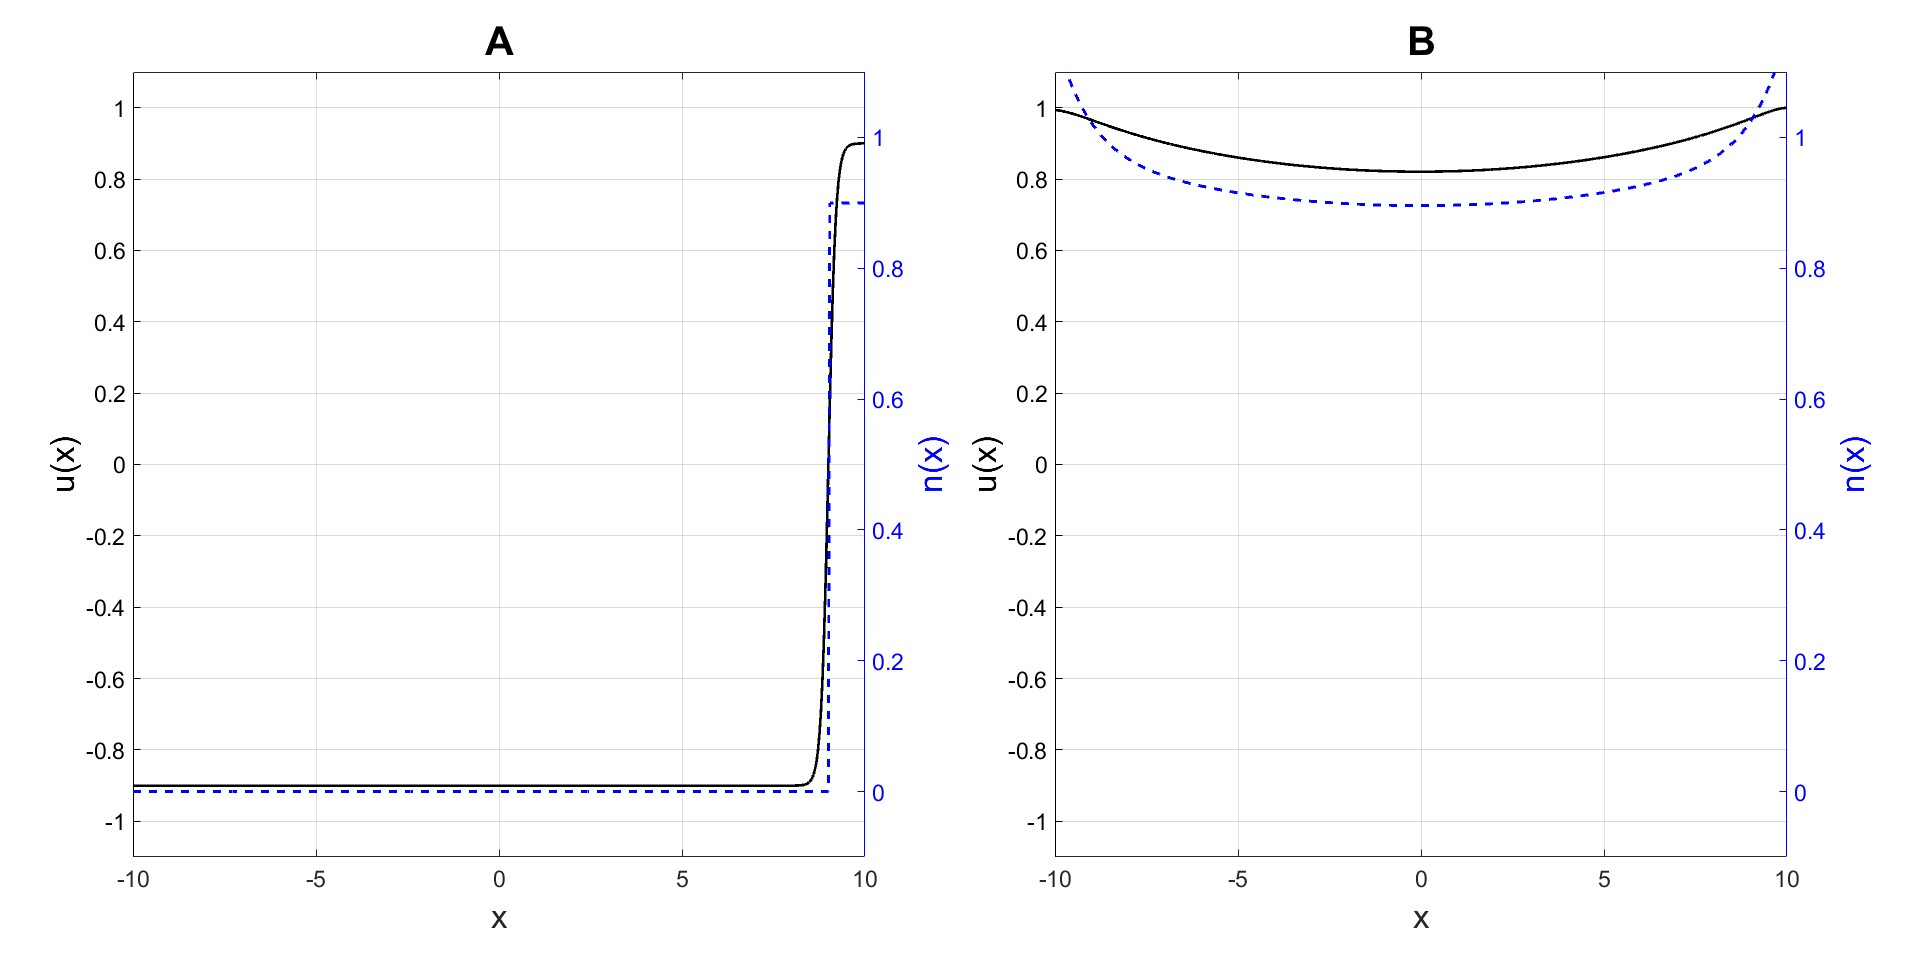
\includegraphics[width=15cm,scale=1]{electron input flux convergence.jpg}
	\caption{Solution with an input electron flux from the right, from the same simulation as Figure \ref{fig:input-flux} . A - initial state, interface around the right edge. B - final state, electron abundance made the $\ce{Ni(OH)_2}$ phase take over the electrode.} \label{fig:output-flux-solution}
\end{figure}

\pagebreak
\section{Conclusions and discussion}

\subsection{Conclusions}
The presented model (\ref{eq:full-model}) went through many changes during this project. As a starting point, we used a different model \hyperref[c:1]{[1]}  to describe the electrode's dynamics. However, I needed to make two major modifications. First, I omitted the positive charge-carrier from the model. Although the nickel-hydroxide reaction (\ref{eq:reaction}) does consist of a positive proton, it is negligible. Second, I changed the electron-material interaction. The proposed model described an attraction between the charge carriers to the phases, but our model had no evidence of such an attraction. Instead, the nickel-hydroxide reaction describes "absorption" of electrons with a phase change, so I added the relevant \hyperref[sec:electron-material]{interaction term}. The acquired knowledge and techniques described above enabled me to modify the original model accordingly.

Although the results of the model successfully describe the basic form of the material's phase change, there are inaccuracies that require further research. Firstly, parameter values in \hyperref[table:1]{Table 1} were set according to physical intuition and are not exact. For example, the permittivity was set high to express the constraining forces that act on the electrons in the material. Secondly, the boundary conditions are not exact - Neumann conditions for $\psi$ cause diverging of the steady state solution, and a potential gradient provided imprecise results (an experiment that details what happens to the physical material under a potential gradient is lacking). Thirdly, I would recommend doing an experiment to check if one phase is energetically favorable to the other (although I found it to be insignificant). Finally, a solution of the model (\ref{eq:full-model}) in two dimensions is needed.


\subsection{Personal experience}
To do this, I needed to study new subjects and train in new skills. Firstly, I needed to study the branch of electrochemistry. Using books, papers, and advises, I built a knowledge basis helped me model the electrode's forces. Secondly, I needed to study Chan-Hilliard's approach to phase separation. It unified a few different subjects from my undergrad studies into one theory, which was interesting yet hard to grasp. Lastly, I needed to study and experiment with different numerical methods for PDE's.

Overall, this project expanded my knowledge and provided me with a taste of research. For the first time, I faced with questions that has no determined answer in the literature, and encountered the combination of different physics theories into one model. The results of the model successfully describe the very basic form of the material's phase change, and provide a starting point for a more detailed and exact model of the electrode and battery.
Finally I would like to thank Professor Arik Yochelis for his much appreciated help and guidance during my work on this project.

\pagebreak
\section{Appendix A - PNP Finite difference} \label{sec:appendix-a}

We would like to solve the following equations (in 1D):

\begin{align}
    \frac{\partial p}{\partial t} &= \nabla^2 p + \nabla(p\nabla \phi) \\
    \frac{\partial n}{\partial t} &= \nabla^2 n - \nabla(n\nabla \phi) \\
    \nabla^2 \phi &= n - p
\end{align}
With the boundary conditions:
\begin{align}
    \nabla p + p \nabla \phi &= \nabla n - n \nabla \phi = 0, \, x=L,0 \\
    \phi(L_x) &= 1, \phi(0) = -1
\end{align}

To find $\phi$ for all $x$ at the current step, I will use the implicit finite difference method.
After applying finite difference, the potential $\phi(x,t)$ at the point $x_m, 0<m<M-1$ would be:

\begin{equation}
    \frac{\Delta x^2}{2}(p_m - n_m) = \phi_m -\frac{1}{2} \phi_{m+1} -\frac{1}{2} \phi_{m-1}
\end{equation}

Therefore, solving for $\phi$ at a certain time would mean solving the following matrix:

\begin{equation}
       \begin{bmatrix}
          1 & -\frac{1}{2} & 0 & 0 & ... \\
          -\frac{1}{2} & 1 & -\frac{1}{2} & 0 & ... \\
          ... & ... \\
          ... & 0 & -\frac{1}{2} & 1 & -\frac{1}{2} \\
          ... & 0 & 0 & -\frac{1}{2} & 1
       \end{bmatrix}
       \begin{bmatrix}
          \phi_1 \\
          \phi_2 \\
          ... \\
          \phi_{M-3} \\
          \phi_{M-2}
       \end{bmatrix}    
         =
         \frac{\Delta x^2}{2}
          \begin{bmatrix}
           p_1 - n_1 + \frac{1}{\Delta x^2} \phi_0 \\
           p_2 - n_2 \\
           ... \\
           p_{M-3} - n_{M-3} \\
           p_{M-2} - n_{M-2} + \frac{1}{\Delta x^2} \phi_M
        
           \end{bmatrix}
\end{equation}

Notice that the LHS matrix is composed of $(M-2)$ ones, and $(M-3)$ elements $-\frac{1}{2}$ on each diagonal.  

Together with finding $\phi$, we need to iterate $p(x,t), n(x,t)$. It means finding $p_m^{i+1}, n_m^{i+1}$. We assume that we have $p_m^j, n_m^j$ for every $m, j<i$.
I will use explicit central difference method to get:

\begin{align}
    \begin{split}
        p_m^{i+1} = {}& p_m^{i} + \frac{\Delta t}{\Delta x^2} [ p_{m+1}^i + p_{m-1}^i - 2p_m^i + \frac{1}{4}(p_{m+1}^i-p_{m-1}^i)(\phi_{m+1}^i-\phi_{m-1}^i) \\
        & + p_m^i(\phi_{m+1}^i+\phi_{m-1}^i-2\phi_m^i) ]
    \end{split} \\
    \begin{split}
        n_m^{i+1} = {}& n_m^{i} + \frac{ \Delta t}{\Delta x^2} [ n_{m+1}^i + n_{m-1}^i - 2n_m^i - \frac{1}{4}(n_{m+1}^i-n_{m-1}^i)(\phi_{m+1}^i-\phi_{m-1}^i) \\
        & - n_m^i(\phi_{m+1}^i+\phi_{m-1}^i-2\phi_m^i) ]
    \end{split}
\end {align}

If we'd like Neumann boundaries, we find:
\begin{align}
    p_0^{i+1} &= \frac{g\Delta x - p_1^{i+1}}{(\phi_1^{i} - \phi_2^{i})-1} \\
    n_0^{i+1} &= \frac{g\Delta x - n_1^{i+1}}{-(\phi_1^{i} - \phi_2^{i})-1} \\
    p_{M-1}^{i+1} &= p_{M-2}^{i+1} - p_{M-2}^{i+1}{(\phi_{M-1}^{i} - \phi_{M-2}^{i})} \\
    n_{M-1}^{i+1} &= n_{M-2}^{i+1} + n_{M-2}^{i+1}{(\phi_{M-1}^{i} - \phi_{M-2}^{i})} 
\end{align}

A full python implementation can be found on this project's \href{https://github.com/nadav7679/phase_field_Ni_batteries/blob/main/pnp_finite_difference.ipynb}{Git repository}

\pagebreak
\section{Bibliography}
[1] Shapira A. Z., Gavish N., Yochelis A., "Pattern formation aspects of electrically charged tristable media with implications to bulk heterojunction in organic photovoltaics", EPL (Europhysics Letters) 125, (2019) 
\label{c:1}
\newline \newline
[2] Allen J. Bard, Larry R. Faulkner, "Electrochemical Methods: Fundamentals and Applications", New York: Wiley, 2001, 2nd ed.. Russian Journal of Electrochemistry 38, 1364–1365 (2002). \label{c:2}
\newline \newline
\href{https://www.phys.uconn.edu/~rozman/Courses/P2200_14F/downloads/cahn-hilliard/docs/spinodal.pdf}{[3]} T. Ursell, “Cahn–Hilliard Kinetics and Spinodal Decomposition in a Diffuse System,” California Institute of Technology (2007) \label{c:3}
\newline \newline
[4] Huggins, R. A., Prinz, H., Wohlfahrtmehrens, M., Jorissen, L., Witschel, W., "Proton Insertion Reactions in Layered Transition-Metal Oxides", Solid State Ionics (1994), 70, 417-424. \label{c:4}
\newline \newline
[5] Srinivasan, V., Weidner, J. W., White, R. E., "Mathematical models of the nickel hydroxide active material", J Solid State Electronics (2000), 4 (7), 367-382. \label{c:5}
\newline \newline
[6] R. Borah, F.R. Hughson, J. Johnston, T. Nann, "On battery materials and methods", Materials Today Advances, Volume 6, (2020) \label{c:6}
\newline \newline
[7] Hongbo Zhao, Richard D. Braatz, Martin Z. Bazant, "Image inversion and uncertainty quantification for constitutive laws of pattern formation", Journal of Computational Physics, (2021), Volume 436 \label{c:7}

\end{document}
